\chapter{Dataset and Complementary Image Data}\label{ch:dataset}

The LiDAR scan I worked with (Ousters OS1-128) provided 3D coordinates, returning intensity values and detected ambient lighting from the surrounding. 

This allowed for consideration of different image projections.

\section{Intensity}{
    
    This information refers to the intensity of the laser beam after being reflected from the respective surface. 
    \begin{figure}[h]
        \centering
        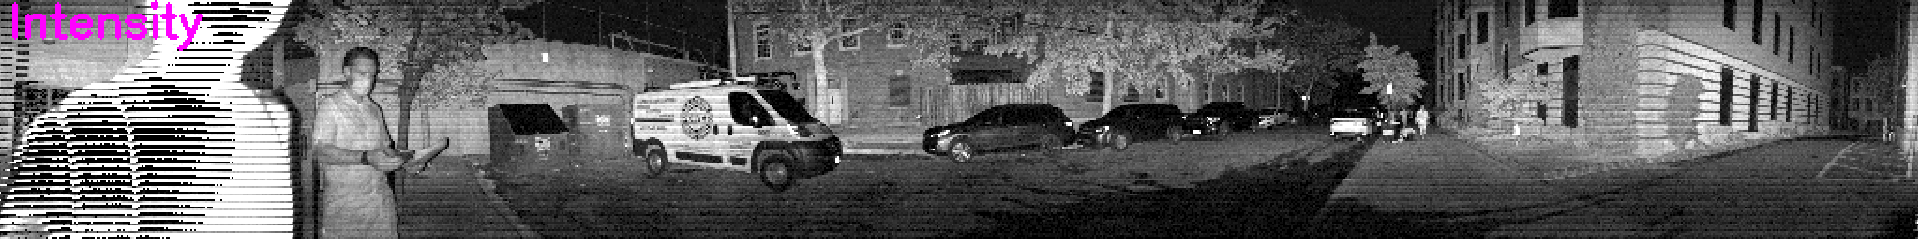
\includegraphics[scale=0.19]{images/dataset/intensity.png}
        \caption{Intensity Image Projection}
        \label{fig:intensity}
    \end{figure}
}

\section{Ambient}{

    The ambient data is the noise lighting from the surrounding. Obviously it is dependent on light however it is the closest to reality of the three data types considered.

    \begin{figure}[h]
        \centering
        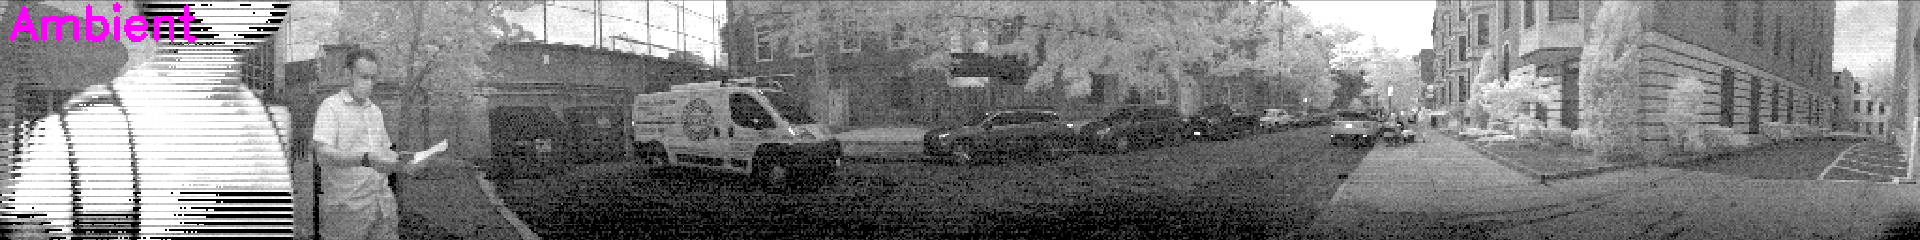
\includegraphics[scale=0.19]{images/dataset/ambient.png}
        \caption{Ambient Image Projection}
        \label{fig:ambient}
    \end{figure}
}
\clearpage

\section{Range}{
    The third data type considered was the depth. Aka each point was assigned a greyscale value depending on its normed distance towards the sensor.\\
    $\text{Range} = \sqrt{p_x^2 + p_y^2 + p_z^2} \quad$ with $p_i$ being the ith coordinate of point p.

    \begin{figure}[h]
        \centering
        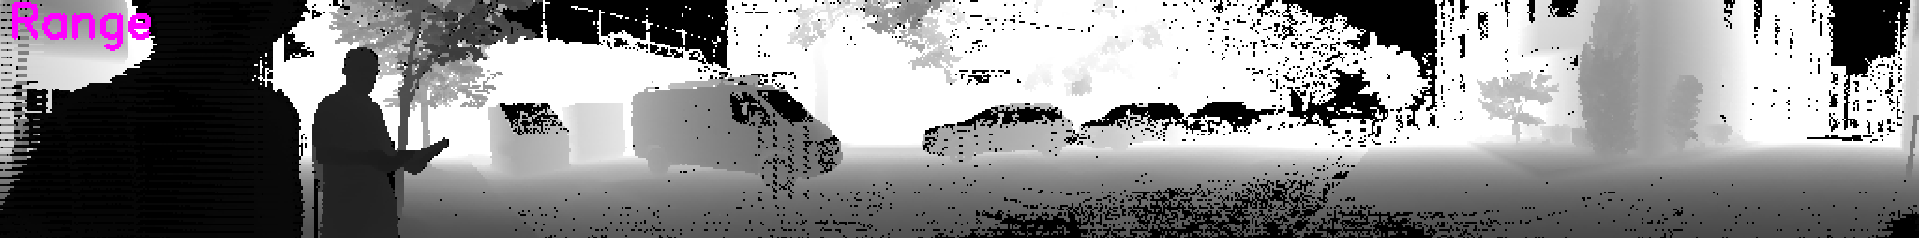
\includegraphics[scale=0.19]{images/dataset/range.png}
        \caption{Range Image Projection}
        \label{fig:range}
    \end{figure}

    
}